\documentclass{article}
% the class can be article, book, and some others; it changes the overall layout of the document

%%%%% preamble starts here %%%%%
% global settings should go into the preamble

% packages and some settings; let's not worry about them now
\usepackage{amsmath, amssymb}
\usepackage{amsthm}
\usepackage{hyperref}
\usepackage{tikz}
% \tikzset{every picture/.style={thick}}
\tikzset{every node/.style={draw, circle, inner sep = 2pt}}
\usetikzlibrary{arrows}

% theorem-type environments; let's not worry about them now
%%%THEOREM
\newtheorem{theorem}{Theorem}[section]
\newtheorem{lemma}[theorem]{Lemma}
\newtheorem{proposition}[theorem]{Proposition}
\newtheorem{corollary}[theorem]{Corollary}

\theoremstyle{definition}
\newtheorem{definition}[theorem]{Definition}
\newtheorem{observation}[theorem]{Observation}
\newtheorem{remark}[theorem]{Remark}
\newtheorem{example}[theorem]{Example}
\newtheorem{notation}[theorem]{Notation}
\newtheorem{question}[theorem]{Question}

% macros; definitions of new commands
\newcommand{\trans}{^\top}
\newcommand{\adj}{^{\rm adj}}
\newcommand{\cof}{^{\rm cof}}
\newcommand{\inp}[2]{\left\langle#1,#2\right\rangle}
\newcommand{\dunion}{\mathbin{\dot\cup}}
\newcommand{\bzero}{\mathbf{0}}
\newcommand{\bone}{\mathbf{1}}
\newcommand{\ba}{\mathbf{a}}
\newcommand{\bb}{\mathbf{b}}
\newcommand{\bp}{\mathbf{p}}
\newcommand{\bq}{\mathbf{q}}
\newcommand{\bx}{\mathbf{x}}
\newcommand{\by}{\mathbf{y}}
\newcommand{\bz}{\mathbf{z}}
\newcommand{\bu}{\mathbf{u}}
\newcommand{\bv}{\mathbf{v}}
\newcommand{\bw}{\mathbf{w}}
\newcommand{\tr}{\operatorname{tr}}
\newcommand{\nul}{\operatorname{null}}
\newcommand{\rank}{\operatorname{rank}}
%\newcommand{\ker}{\operatorname{ker}}
\newcommand{\range}{\operatorname{range}}
\newcommand{\Col}{\operatorname{Col}}
\newcommand{\Row}{\operatorname{Row}}
\newcommand{\spec}{\operatorname{spec}}
\newcommand{\vspan}{\operatorname{span}}
%%%%% preamble ends here %%%%%

% all content should go into the document environment
\begin{document}

Use \href{https://katex.org/docs/supported.html}{KaTeX: Supported Functions} and \href{https://sagelabtw.github.io/LA-Tea/style.html}{LA Tea-style} to check out the commands, if necessary.  Type the following paragraphs:
\medskip

%%% remove from here
% inline math
% display math
Consider the equation $x^2 + x + 1 = 0$.  One may use the quadratic formula to find the zeros  
\[\frac{-1+\sqrt{3}}{2} \text{ and } \frac{-1-\sqrt{3}}{2}.\]

Let 
\[A = \begin{bmatrix}
 1 & 2 & 3 \\
 4 & 5 & 6 \\
 7 & 8 & 9
\end{bmatrix}.\]
Then $A\bv = \bzero$ is equivalent to the system of linear equations
\[\begin{aligned}
 x + 2y + 3z &= 0, \\
 4x + 5y + 6z &= 0, \\
 7x + 8y + 9z &= 0.
\end{aligned}\]

Notice that every sentence is \textbf{complete} and \emph{with proper punctuation marks}.
%%% remove to here

\bigskip

Based on the code provided below, draw the first letter of your last name, and use the arrows to indicate how the letter should be written.  Add a loop to at least one of the vertices.
\medskip

\begin{center}
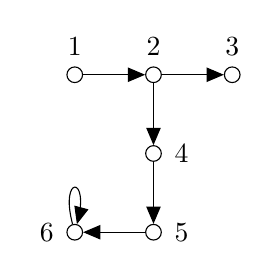
\begin{tikzpicture}
\node[label={above:$1$}] (1) at (0,2) {};
\node[label={above:$2$}] (2) at (1,2) {};
\node[label={above:$3$}] (3) at (2,2) {};
\node[label={right:$4$}] (4) at (1,1) {};
\node[label={right:$5$}] (5) at (1,0) {};
\node[label={left:$6$}] (6) at (0,0) {};
    
\draw[-triangle 45] (1) -- (2);
\draw[-triangle 45] (2) -- (3);
\draw[-triangle 45] (2) -- (4);
\draw[-triangle 45] (4) -- (5);
\draw[-triangle 45] (5) -- (6);
\draw[-triangle 45] (6) to [loop above, looseness=30] (6);
\end{tikzpicture}
\end{center}


\end{document}